\documentclass{article}
\usepackage{fancyhdr}
\usepackage[utf8]{inputenc}
\usepackage[english]{babel}
\usepackage{tikz, multicol, graphicx, etoolbox, enumerate, setspace, relsize, mathrsfs, verbatim}
\usepackage{amsmath, amsfonts, amssymb, amsthm, epsfig, epstopdf, titling, url, array, esvect, tikz-3dplot}
\usepackage{graphicx}
\usepackage{hyperref}

\usepackage{listings}
\usepackage{xcolor}

\definecolor{codegreen}{rgb}{0,0.6,0}
\definecolor{codegray}{rgb}{0.5,0.5,0.5}
\definecolor{codepurple}{rgb}{0.58,0,0.82}
\definecolor{backcolour}{rgb}{0.95,0.95,0.92}

\usepackage{pgfplots}
\usepackage{tcolorbox}
\usepackage{amsthm}
\usepackage{cancel}
\usepackage[left=1in,right=1in,top=1in,bottom=1in]{geometry}
\usepackage[tableaux]{prooftrees}

\lstdefinestyle{mystyle}{
    backgroundcolor=\color{backcolour},   
    commentstyle=\color{codegreen},
    keywordstyle=\color{magenta},
    numberstyle=\tiny\color{codegray},
    stringstyle=\color{codepurple},
    basicstyle=\ttfamily\footnotesize,
    breakatwhitespace=false,         
    breaklines=true,                 
    captionpos=b,                    
    keepspaces=true,                 
    numbers=left,                    
    numbersep=5pt,                  
    showspaces=false,                
    showstringspaces=false,
    showtabs=false,                  
    tabsize=2
}

\lstset{style=mystyle}

\pagestyle{fancy}
\fancyhf{}
\fancyhead[L,RO]{Tasksheet 6}
\fancyhead[R,RO]{Fundamentals of Computational Mathematics}
\fancyfoot[L,RO]{Xiang Gao}
\fancyfoot[R,RO]{Math 4610}
\renewcommand{\headrulewidth}{0.4pt}% Default \headrulewidth is 0.4pt
\renewcommand{\footrulewidth}{0.4pt}% Default \footrulewidth is 0pt
\def\checkmark{\tikz\fill[scale=0.4](0,.35) -- (.25,0) -- (1,.7) -- (.25,.15) -- cycle;} 

\begin{document}

\section*{Task 1}
I have created the following testing python file for this test. And the python module folder can be found \href{https://github.com/GoByMark/math4610/tree/main/Homework_Tasks/Tasksheet_06/src/Task_1/mypythonlib}{here}.
\lstinputlisting[language=Python]{Task_1/mypythonlib/test.py}
These are the results I have found using the four different methods that are closed to zero. I have included two results, since when I ran the code from terminal, the fixed point method didn't converge while as running from the IDE shows it does converge.
\begin{center}
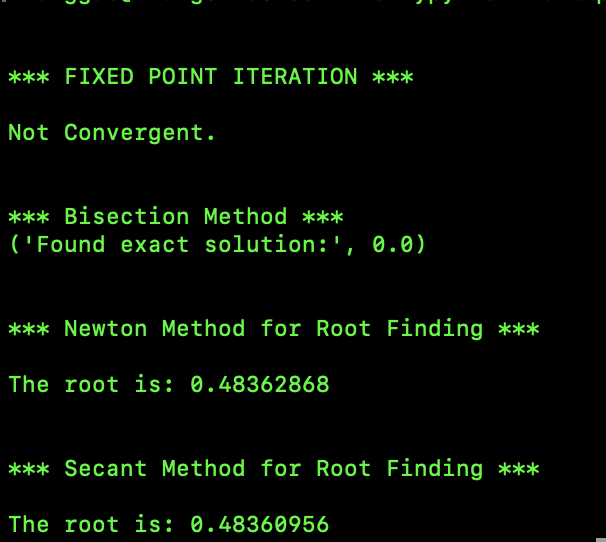
\includegraphics[width=0.4\textwidth]{Screenshots/Task_1.1.png}
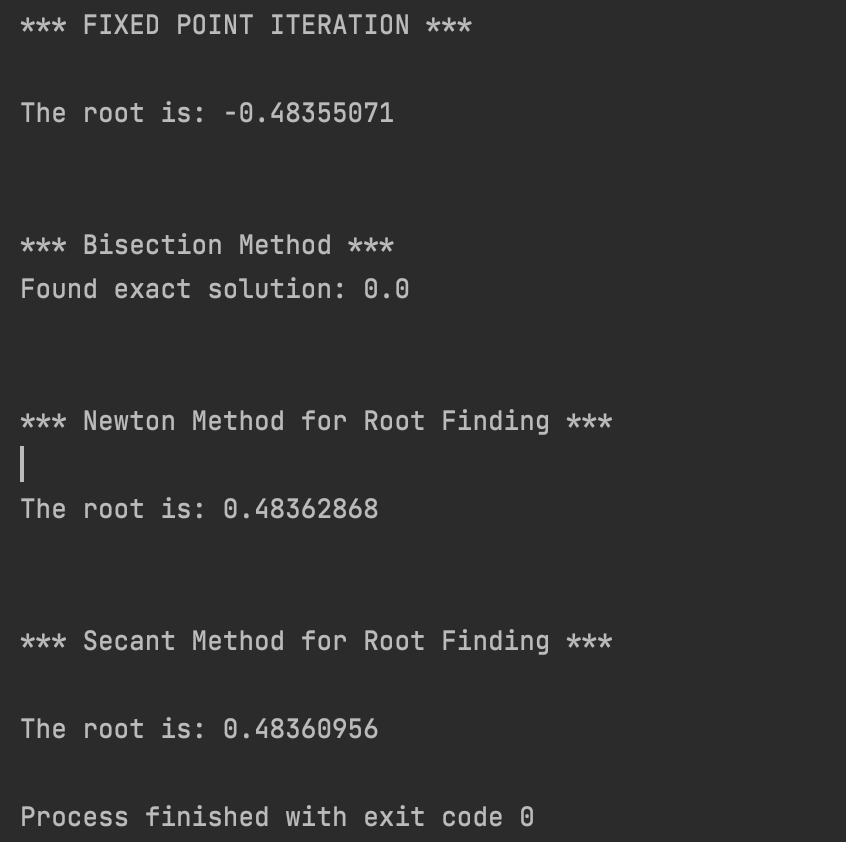
\includegraphics[width=0.4\textwidth]{Screenshots/Task_1.2.png}\\
{\bf Figure 1.} Running the Test Code from the Terminal vs. Running from the IDE.
\end{center}

\section*{Task 2}
Using my Newton method with $x_0 = -5.0$ and $x_0 = 6$, given the following code:
\lstinputlisting[language=Python]{Task_2.py}
We have the following two results, for $x_0 = -5.0$ and $x_0 = 6$, respectively.
\begin{center}
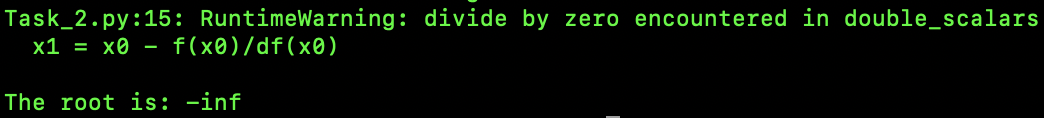
\includegraphics[width=\textwidth]{Screenshots/Task_2.1.png}
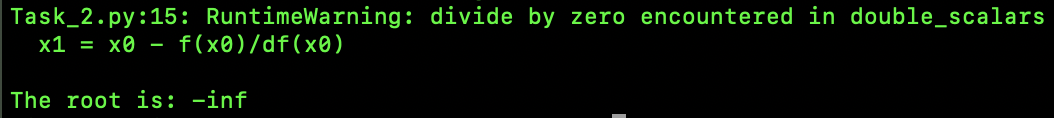
\includegraphics[width=\textwidth]{Screenshots/Task_2.2.png}\\
{\bf Figure 2.} The Results Using Newton Method With $x_0 = -5.0$ and $x_0 = 6$, Respectively.
\end{center}
Comparing to Task $1$, the problem comes with the large initial guess.

\section*{Task 3}
Using my updated hybird method with the initial interval $[-5, 6]$, 
\lstinputlisting[language=Python]{Task_3.py}
I get the following result
\begin{center}
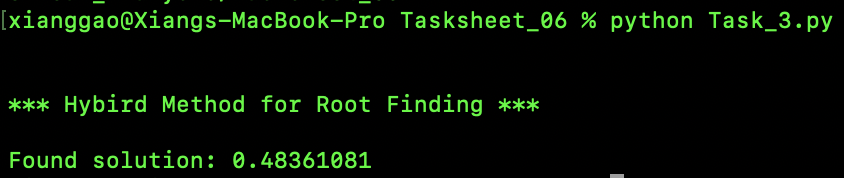
\includegraphics[width=\textwidth]{Screenshots/Task_3.png}
{\bf Figure 3.} The Results Using Hybird Method with the Initial Interval $[-5, 6]$.
\end{center}

\section*{Task 4}
The following code is the hybrid method using the secant method, however, I wasn't able to fix the code in time to before the due time.
\lstinputlisting[language=Python]{Task_4.py}

\section*{Task 6}
From this \href{http://jwilson.coe.uga.edu/EMT669/Student.Folders/Frietag.Mark/Homepage/roots/roots.html}{website}\footnote{http://jwilson.coe.uga.edu/EMT669/Student.Folders/Frietag.Mark/Homepage/roots/roots.html} I found, when it comes to finding multiple roots of a function. It's really hard to come up with a structural algorithmic approach.\\
However, with the information from \href{https://www.ams.org/journals/mcom/1965-19-092/S0025-5718-1965-0198670-6/}{this website}\footnote{https://www.ams.org/journals/mcom/1965-19-092/S0025-5718-1965-0198670-6/}. The Broyden's method is apparently one approach for function with multiple roots.
\end{document}